\documentclass[12pt]{article}
\usepackage[a4paper,margin=2.5cm]{geometry}
\usepackage{amsmath, amsfonts, amssymb, amsthm}
\usepackage{physics}
\usepackage{mathtools}
\usepackage{tikz}
\usetikzlibrary{decorations.pathreplacing}
\newtheorem{theorem}{Teorema}

\title{Teoremas}
\author{Juan Rodríguez}
\date{}
\begin{document}
\maketitle
\section*{Demostrar que la composición de dos funciones continuas es continua}

Sean \( f : X \to Y \) y \( g : Y \to Z \) dos funciones continuas.  
Queremos demostrar que \( g \circ f : X \to Z \) también es continua. \\

\begin{center}
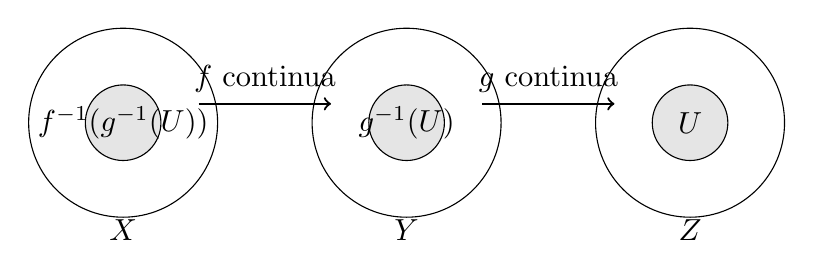
\begin{tikzpicture}[scale=1.2, every node/.style={scale=1.1}]
    % Conjuntos
    \draw (0,0) circle (1cm) node[below=1cm] {$X$};
    \draw (3,0) circle (1cm) node[below=1cm] {$Y$};
    \draw (6,0) circle (1cm) node[below=1cm] {$Z$};

    % Flechas
    \draw[->, thick] (0.8,0.2) -- (2.2,0.2) node[midway, above] {$f$ continua};
    \draw[->, thick] (3.8,0.2) -- (5.2,0.2) node[midway, above] {$g$ continua};

    % Conjuntos interiores
    \draw[fill=gray!20] (6,0) circle (0.4cm) node {\(U\)};
    \draw[fill=gray!20] (3,0) circle (0.4cm) node {\(g^{-1}(U)\)};
    \draw[fill=gray!20] (0,0) circle (0.4cm) node {\(f^{-1}(g^{-1}(U))\)};
\end{tikzpicture}
\end{center}

\noindent
Sea \( U \subseteq Z \) un conjunto abierto.  
Como \( g \) es continua, se cumple que \( g^{-1}(U) \) es abierto en \(Y\).  
Como \( f \) es continua, la preimagen \( f^{-1}(g^{-1}(U)) \) es abierta en \(X\).

Por lo tanto, la preimagen de un abierto por la composición \( g \circ f \) es abierta:
\[
(g \circ f)^{-1}(U) = f^{-1}(g^{-1}(U)),
\]
y así \( g \circ f \) es continua.

\section*{Demostrar que la distancia euclidiana, la del máximo y la taxicab son equivalentes}

\subsection*{Definiciones de las tres distancias en $\mathbb{R}^2$}
\[
d_E(x,y) = \sqrt{(x_1 - y_1)^2 + (x_2 - y_2)^2}, \quad
d_T(x,y) = |x_1 - y_1| + |x_2 - y_2|, \quad
d_M(x,y) = \max\{|x_1 - y_1|, |x_2 - y_2|\}.
\]

\subsection*{Bolas abiertas en cada distancia}
\begin{center}
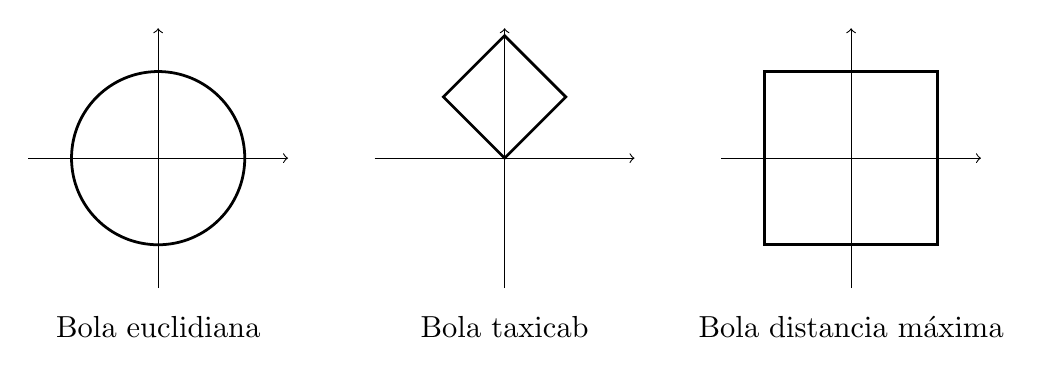
\begin{tikzpicture}[scale=1.1, every node/.style={scale=1.1}]
  % Euclidiana
  \begin{scope}[shift={(-4,0)}]
    \draw[->] (-1.5,0)--(1.5,0);
    \draw[->] (0,-1.5)--(0,1.5);
    \draw[line width=1pt] (0,0) circle (1cm);
    \node[below=1.7cm] at (0,0) {Bola euclidiana};
  \end{scope}

  % Taxicab
  \begin{scope}[shift={(0,0)}]
    \draw[->] (-1.5,0)--(1.5,0);
    \draw[->] (0,-1.5)--(0,1.5);
    \draw[line width=1pt, rotate=45] (0,0) rectangle (1cm,1cm);
    \node[below=1.7cm] at (0,0) {Bola taxicab};
  \end{scope}

  % Máximo
  \begin{scope}[shift={(4,0)}]
    \draw[->] (-1.5,0)--(1.5,0);
    \draw[->] (0,-1.5)--(0,1.5);
    \draw[line width=1pt] (-1,-1) rectangle (1,1);
    \node[below=1.7cm] at (0,0) {Bola distancia máxima};
  \end{scope}
\end{tikzpicture}
\end{center}

\subsection*{Demostramos que las distancias son equivalentes}

\paragraph{1. Euclidiana y Taxicab.}
Dentro de toda bola abierta de la distancia euclidiana existe una bola abierta de la distancia taxicab, y viceversa.
Por tanto, las topologías inducidas por ambas distancias coinciden.

\[
\exists\, c_1, c_2 > 0 \text{ tales que } c_1\,d_E(x,y) \le d_T(x,y) \le c_2\,d_E(x,y).
\]
De hecho, en $\mathbb{R}^2$, se cumple \( d_E(x,y) \le d_T(x,y) \le \sqrt{2}\,d_E(x,y) \).

\begin{center}
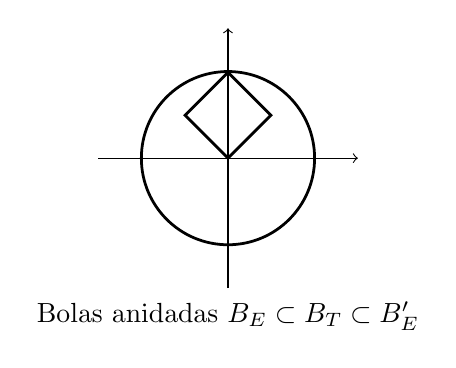
\begin{tikzpicture}[scale=1.1]
  \draw[->] (-1.5,0)--(1.5,0);
  \draw[->] (0,-1.5)--(0,1.5);
  \draw[line width=1pt] (0,0) circle (1cm);
  \draw[line width=1pt, rotate=45] (0,0) rectangle (0.7cm,0.7cm);
  \node[below=1.7cm] at (0,0) {Bolas anidadas $B_E \subset B_T \subset B_E'$};
\end{tikzpicture}
\end{center}

\paragraph{2. Taxicab y Máxima.}
De forma análoga, dentro de toda bola abierta de la distancia taxicab
hay una bola abierta de la distancia máxima y viceversa.
\[
d_M(x,y) \le d_T(x,y) \le 2\,d_M(x,y),
\]
por lo que son equivalentes.

\begin{center}
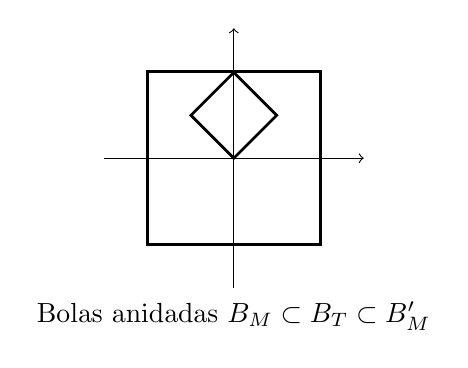
\begin{tikzpicture}[scale=1.1]
  \draw[->] (-1.5,0)--(1.5,0);
  \draw[->] (0,-1.5)--(0,1.5);
  \draw[line width=1pt] (-1,-1) rectangle (1,1);
  \draw[line width=1pt, rotate=45] (0,0) rectangle (0.7cm,0.7cm);
  \node[below=1.7cm] at (0,0) {Bolas anidadas $B_M \subset B_T \subset B_M'$};
\end{tikzpicture}
\end{center}

\paragraph{3. Euclidiana y Máxima.}
Como ambas son equivalentes a la taxicab, también son equivalentes entre sí.  
Por tanto:
\[
\boxed{\text{Euclidiana } \equiv \text{ Taxicab } \equiv \text{ Máxima}}
\]

\begin{center}
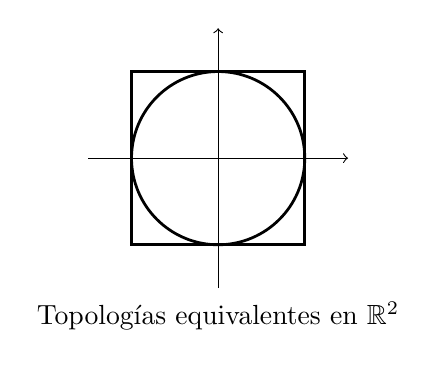
\begin{tikzpicture}[scale=1.1]
  \draw[->] (-1.5,0)--(1.5,0);
  \draw[->] (0,-1.5)--(0,1.5);
  \draw[line width=1pt] (0,0) circle (1cm);
  \draw[line width=1pt] (-1,-1) rectangle (1,1);
  \node[below=1.7cm] at (0,0) {Topologías equivalentes en $\mathbb{R}^2$};
\end{tikzpicture}
\end{center}
\section*{Demostrar que dos distancias equivalentes generan una topología equivalente}

Queremos demostrar que si dos distancias \( d_1 \) y \( d_2 \) sobre un mismo conjunto \( X \)
son \textbf{equivalentes}, entonces inducen la misma topología, es decir,
los conjuntos abiertos en una son también abiertos en la otra y viceversa.

\subsection*{Definición de distancias equivalentes}
Decimos que \( d_1 \) y \( d_2 \) son equivalentes si:
\[
\forall x \in X, \ \forall \varepsilon > 0, \ \exists \delta_1 > 0, \ \exists \delta_2 > 0
\]
tales que:
\[
B_{d_1}(x, \delta_1) \subseteq B_{d_2}(x, \varepsilon)
\quad \text{y} \quad
B_{d_2}(x, \delta_2) \subseteq B_{d_1}(x, \varepsilon).
\]

Es decir, las bolas abiertas de una métrica pueden ser contenidas dentro
de las bolas abiertas de la otra, y viceversa.

\subsection*{Demostración}
Sea \( x \in X \) y \( \varepsilon > 0 \).
Por equivalencia de las distancias, existen \( \delta_1, \delta_2 > 0 \) tales que:

\begin{itemize}
  \item Si \( y \in X \) y \( d_1(x,y) < \delta_1 \), entonces \( d_2(x,y) < \varepsilon \).
  \item Si \( y \in X \) y \( d_2(x,y) < \delta_2 \), entonces \( d_1(x,y) < \varepsilon \).
\end{itemize}

Por tanto:
\[
B_{d_1}(x, \delta_1) \subseteq B_{d_2}(x, \varepsilon)
\quad \text{y} \quad
B_{d_2}(x, \delta_2) \subseteq B_{d_1}(x, \varepsilon).
\]

Esto implica que:
\begin{itemize}
    \item Si un conjunto \(U\) es abierto en la métrica \(d_1\), entonces para cada \(x \in U\)
    existe una bola \(B_{d_1}(x, \delta_1) \subseteq U\).  
    Como \(B_{d_1}(x, \delta_1) \subseteq B_{d_2}(x, \varepsilon)\),
    el conjunto \(U\) también es abierto en la métrica \(d_2\).

    \item De manera simétrica, si \(U\) es abierto en \(d_2\),
    también lo es en \(d_1\).
\end{itemize}

\subsection*{Conclusión}
Como los conjuntos abiertos son los mismos en ambas métricas:
\[
\boxed{\mathcal{T}(d_1) = \mathcal{T}(d_2)}
\]
Por lo tanto, \(d_1\) y \(d_2\) generan la misma topología, llamada \textbf{topología equivalente}.
\section*{En $\mathbb{R}$, toda base puede reducirse}

Sea $\mathcal{B}$ una base de la topología canónica en $\mathbb{R}$, por ejemplo
la familia de todos los intervalos abiertos $(a,b)$ con $a<b$.

\subsection*{Idea general}
Una base $\mathcal{B}$ se dice \textbf{reducible} si existe algún elemento
$B \in \mathcal{B}$ que puede escribirse como unión de otros elementos de la base, es decir:
\[
B = \bigcup_{i \in I} B_i, \quad \text{con } B_i \in \mathcal{B} \setminus \{B\}.
\]
En ese caso, $B$ es redundante y puede eliminarse sin modificar la topología generada.

\subsection*{Ejemplo intuitivo}
Sean los intervalos
\[
B_1 = (3,5), \qquad B_2 = (2,7).
\]
Como $B_1 \subseteq B_2$, el conjunto $B_1$ no aporta nueva información topológica.
En efecto, cualquier abierto que contenga a $(3,5)$ puede expresarse como unión
de intervalos abiertos que contienen a $(3,5)$, por ejemplo
\[
(3,5) = (2,5) \cap (3,7),
\]
y ambos intervalos también son abiertos en $\mathbb{R}$.
Por tanto, $B_1$ puede eliminarse de la base sin alterar la topología.

\subsection*{Reducción general}
Sea $A \subseteq \mathbb{R}$ un conjunto abierto.
Por definición de base, se puede expresar como unión de elementos de $\mathcal{B}$:
\[
A = \bigcup_{B_i \in \mathcal{B}_A} B_i,
\]
donde $\mathcal{B}_A \subseteq \mathcal{B}$.
Si existe $B_j \in \mathcal{B}_A$ tal que $B_j \subseteq \bigcup_{i \ne j} B_i$,
entonces $B_j$ es redundante y puede eliminarse sin modificar la unión.

Así, definimos la base reducida:
\[
\mathcal{B}' = \mathcal{B} \setminus \{B_j : B_j \subseteq \bigcup_{i \ne j} B_i\}.
\]
La familia $\mathcal{B}'$ genera la misma topología que $\mathcal{B}$,
ya que toda bola abierta o intervalo de $\mathcal{B}$ está contenida en una unión de elementos de $\mathcal{B}'$.

\subsection*{Conclusión}
En $\mathbb{R}$, toda base de la topología canónica puede reducirse eliminando los elementos redundantes,
pues cada intervalo abierto puede ser cubierto por la unión de otros intervalos abiertos de la base.
Además, puede obtenerse una base numerable reducida tomando sólo intervalos con extremos racionales:
\[
\mathcal{B}_\mathbb{Q} = \{(a,b) : a,b \in \mathbb{Q},\ a<b\}.
\]
Por tanto, $\mathbb{R}$ admite una base reducida y numerable para su topología canónica.
\section*{Continuidad de la identidad y relación entre topologías}

\begin{theorem}
Sea $X$ un conjunto y $T,T'$ dos topologías sobre $X$.
La función identidad
\[
\operatorname{id}:(X,T)\longrightarrow (X,T'),\qquad \operatorname{id}(x)=x,
\]
es continua \emph{si y sólo si} $T'\subseteq T$ (es decir, $T'$ es más \emph{gruesa} o igual que $T$).
\end{theorem}

\begin{proof}
($\Rightarrow$) Supongamos que $\operatorname{id}:(X,T)\to (X,T')$ es continua.
Sea $U\in T'$ un abierto del espacio de llegada. Por continuidad,
$\operatorname{id}^{-1}(U)$ debe ser abierto en el espacio de partida $(X,T)$.
Pero $\operatorname{id}^{-1}(U)=U$. Luego $U\in T$.
Como esto vale para todo $U\in T'$, concluimos $T'\subseteq T$.

($\Leftarrow$) Supongamos ahora que $T'\subseteq T$.
Tomemos $U\in T'$; entonces $U\in T$ por la hipótesis.
Como $\operatorname{id}^{-1}(U)=U\in T$, la preimagen de todo abierto de $(X,T')$
es abierta en $(X,T)$, y por tanto $\operatorname{id}:(X,T)\to (X,T')$ es continua.
\end{proof}
\section*{$f$ es continua $\iff$ la preimagen de un abierto es abierta}

Sean $(X,d_X)$ y $(Y,d_Y)$ espacios métricos y $f:X\to Y$.

\subsection*{($\Rightarrow$) Si $f$ es continua, entonces $f^{-1}(U)$ es abierta para toda $U\subseteq Y$ abierta}
Sea $U\subseteq Y$ un abierto. Supondremos, por reducción al absurdo, que $f^{-1}(U)$ \emph{no} es abierta.
Entonces existe $x\in f^{-1}(U)$ que es \textbf{punto frontera} de $f^{-1}(U)$; equivalentemente,
existe una sucesión $(x_n)\subset X\setminus f^{-1}(U)$ tal que $x_n\to x$ en $X$.
(Geométricamente: puntos $x_n$ que se acercan a $x$ pero \emph{desde fuera} de la preimagen.)

\begin{center}
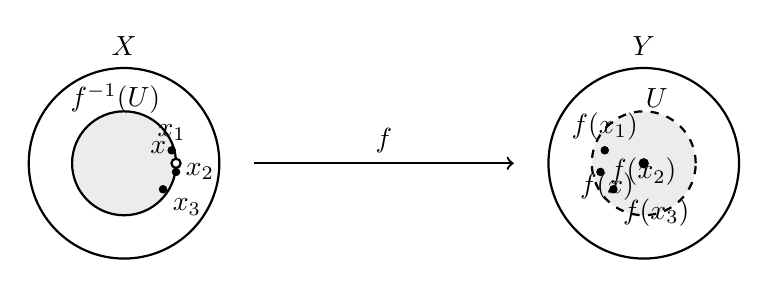
\begin{tikzpicture}[scale=1.1]

% --- Dominio X ---
\draw[thick] (-3,0) circle (1.1);
\node at (-3,1.35) {$X$};

% conjunto f^{-1}(U) -- cerrado o no abierto
\filldraw[fill=gray!15,draw=black,thick] (-3,0) circle (0.6);
\node at (-3.1,0.75) {$f^{-1}(U)$};

% puntos x_i fuera del conjunto pero cerca del borde
\filldraw (-2.45,0.15) circle (1.2pt) node[above] {$x_1$};
\filldraw (-2.4,-0.1) circle (1.2pt) node[right] {$x_2$};
\filldraw (-2.55,-0.3) circle (1.2pt) node[below right] {$x_3$};

% punto x en la frontera (dibujado sobre el borde)
\filldraw[fill=white,draw=black,thick] (-2.4,0) circle (1.5pt);
\node[above left] at (-2.4,0) {$x$};

% --- Codominio Y ---
\draw[thick] (3,0) circle (1.1);
\node at (3,1.35) {$Y$};

% conjunto U -- abierto (línea discontinua)
\filldraw[fill=gray!15,draw=none] (3,0) circle (0.6);
\draw[dashed,thick] (3,0) circle (0.6);
\node at (3.15,0.75) {$U$};

% imágenes de los puntos
\filldraw (2.55,0.15) circle (1.2pt) node[above] {$f(x_1)$};
\filldraw (2.5,-0.1) circle (1.2pt) node[right] {$f(x_2)$};
\filldraw (2.65,-0.3) circle (1.2pt) node[below right] {$f(x_3)$};

% imagen del punto x, en el interior del abierto
\filldraw (3,0) circle (1.5pt) node[below left] {$f(x)$};

% flecha entre los dos espacios
\draw[->,thick] (-1.5,0) -- (1.5,0) node[midway,above] {$f$};

\end{tikzpicture}

\smallskip
\textit{El conjunto $f^{-1}(U)$ (línea continua) no es abierto, y $x$ está en su frontera. 
Los puntos $x_i$ se aproximan a $x$ desde fuera, pero las imágenes $f(x_i)$ se aproximan a $f(x)$ dentro de $U$ (línea discontinua), 
lo que contradice que $f(x)$ fuera frontera.}
\end{center}



Como $x\in f^{-1}(U)$, tenemos $f(x)\in U$. Al ser $U$ abierto, existe $\varepsilon>0$ con
$B_Y(f(x),\varepsilon)\subset U$. Por continuidad de $f$ en $x$, existe $\delta>0$ tal que
\[
d_X(x_n,x)<\delta \ \Longrightarrow\ d_Y\bigl(f(x_n),f(x)\bigr)<\varepsilon
\ \Longrightarrow\ f(x_n)\in B_Y(f(x),\varepsilon)\subset U.
\]
Pero $x_n\notin f^{-1}(U)$ para todo $n$, es decir, $f(x_n)\notin U$, lo cual contradice la conclusión anterior.
La contradicción muestra que $f^{-1}(U)$ debe ser abierta.

\subsection*{($\Leftarrow$) Si la preimagen de todo abierto es abierta, entonces $f$ es continua}
Supongamos que para todo abierto $V\subseteq Y$, el conjunto $f^{-1}(V)$ es abierto en $X$.
Sea $x\in X$ y sea $\varepsilon>0$. El conjunto $V:=B_Y(f(x),\varepsilon)$ es abierto en $Y$; por hipótesis,
$f^{-1}(V)$ es abierto en $X$ y contiene a $x$. Luego existe $\delta>0$ tal que
\[
B_X(x,\delta)\subset f^{-1}\bigl(B_Y(f(x),\varepsilon)\bigr).
\]
Así, si $d_X(x,y)<\delta$ entonces $y\in f^{-1}(V)$ y por tanto
$d_Y\bigl(f(y),f(x)\bigr)<\varepsilon$. Esto verifica la continuidad de $f$ en $x$.
Como $x$ era arbitrario, $f$ es continua en todo $X$.

\section*{\(f \text{ es continua en } x \quad \Longleftrightarrow \quad
\text{para toda sucesión } (x_n)\subset X \text{ con } x_n \to x,\ \ f(x_n) \to f(x).\)}

Sean $(X,d_X)$ y $(Y,d_Y)$ espacios métricos y $f:X\to Y$. Para $x\in X$ se tiene:

\subsection*{($\Rightarrow$) Si $f$ es continua en $x$, entonces conserva convergencia de sucesiones en $x$}
Sea $(x_n)$ tal que $x_n\to x$. Dado $\varepsilon>0$, por continuidad en $x$ existe $\delta>0$ con
\[
d_X(x_n,x)<\delta \ \Longrightarrow\ d_Y(f(x_n),f(x))<\varepsilon.
\]
Como $x_n\to x$, existe $N$ tal que $d_X(x_n,x)<\delta$ para todo $n\ge N$; por tanto
$d_Y(f(x_n),f(x))<\varepsilon$ para todo $n\ge N$. Luego $f(x_n)\to f(x)$.

\subsection*{($\Leftarrow$) Si $f$ conserva convergencia de sucesiones en $x$, entonces es continua en $x$}
Demostraremos la contraposición. Supongamos que $f$ \emph{no} es continua en $x$. Entonces existe
$\varepsilon_0>0$ tal que para todo $\delta>0$ se puede elegir $y\in X$ con
\[
d_X(y,x)<\delta \quad \text{y} \quad d_Y\big(f(y),f(x)\big)\ge \varepsilon_0.
\]
Tomando $\delta=\tfrac{1}{n}$, elegimos $y_n\in X$ con
\[
d_X(y_n,x)<\tfrac{1}{n}
\quad\text{y}\quad
d_Y\big(f(y_n),f(x)\big)\ge \varepsilon_0 \quad \text{para todo } n.
\]
Entonces $y_n\to x$, pero $(f(y_n))$ \emph{no} converge a $f(x)$. Esto contradice la hipótesis de conservación de convergencia.
Por tanto, $f$ debe ser continua en $x$.

\section*{Teorema del Punto Fijo de Banach}

\textbf{Enunciado.}  
Sea $(X,d)$ un espacio métrico completo y sea $f:X\to X$ una \textbf{contracción}, es decir,
existe una constante $0 < c < 1$ tal que:
\[
d(f(x),f(y)) \leq c\,d(x,y), \quad \forall x,y\in X.
\]
Entonces:\\
1. Existe un único punto fijo $x^*\in X$ tal que $f(x^*)=x^*$. \\
2. Para cualquier $x_0\in X$, la sucesión definida por:
\[
x_{n+1}=f(x_n)
\]
converge a dicho punto fijo.

\subsection*{Unicidad del punto fijo}
Supongamos que existen dos puntos fijos $a,b\in X$ tales que $f(a)=a$ y $f(b)=b$.  
Entonces:
\[
d(a,b) = d(f(a),f(b)) \leq c\,d(a,b).
\]
Como $0<c<1$, esto solo es posible si $d(a,b)=0$, es decir, $a=b$.  
Por tanto, el punto fijo, si existe, es \textbf{único}.

\subsection*{Existencia del punto fijo}
Definimos la sucesión $\{x_n\}$ por:
\[
x_{n+1} = f(x_n), \quad n\ge 0.
\]
Queremos demostrar que $\{x_n\}$ es de Cauchy.

Sea $m>n$.  
Aplicando la desigualdad contractiva repetidamente, se obtiene:
\[
\begin{aligned}
d(x_{n+m},x_n)
&\le d(x_{n+m},x_{n+m-1}) + d(x_{n+m-1},x_{n+m-2}) + \dots + d(x_{n+1},x_n) \\
&\le c^{n+m-1}d(x_1,x_0) + c^{n+m-2}d(x_1,x_0) + \dots + c^n d(x_1,x_0) \\
&\le c^n\,d(x_1,x_0)\,\frac{1-c^m}{1-c}.
\end{aligned}
\]
Como $0<c<1$, cuando $n\to\infty$ se tiene:
\[
d(x_{n+m},x_n) \le \frac{c^n}{1-c}d(x_1,x_0) \longrightarrow 0.
\]
Por tanto, $\{x_n\}$ es una sucesión de Cauchy.  
Como $X$ es completo, existe $x^*\in X$ tal que $x_n\to x^*$.

\subsection*{Comprobación de que $x^*$ es punto fijo}
Por continuidad de $f$ (la contracción es continua),
\[
f(x^*) = f\left(\lim_{n\to\infty}x_n\right)
= \lim_{n\to\infty} f(x_n)
= \lim_{n\to\infty} x_{n+1}
= x^*.
\]
Por tanto, $x^*$ es punto fijo.  

\subsection*{Conclusión}
La función $f$ tiene un único punto fijo $x^*\in X$, y para cualquier $x_0\in X$, la sucesión
definida por $x_{n+1}=f(x_n)$ converge a él.
\section*{Todo conjunto cerrado coincide con su clausura}

Sea $C \subset X$.  
Queremos demostrar que:
\[
C \text{ es cerrado } \quad \Longleftrightarrow \quad \overline{C} = C.
\]

\subsection*{($\Rightarrow$) Si $C$ es cerrado, entonces $C = \overline{C}$}
Por definición, $C$ es cerrado si su complementario $X \setminus C$ es abierto.  
Supongamos, por reducción al absurdo, que existe un punto $x \in \overline{C}$ tal que $x \notin C$.

Entonces $x \in X \setminus C$, y como $X \setminus C$ es abierto, existe una bola abierta
$B(x,\varepsilon)$ tal que:
\[
B(x,\varepsilon) \subset X \setminus C.
\]
Pero esto contradice el hecho de que $x \in \overline{C}$, ya que todo entorno de $x$
debería intersectar a $C$.  

\begin{center}
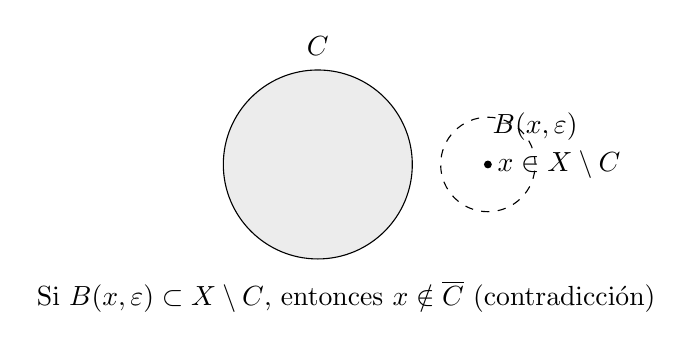
\begin{tikzpicture}[scale=1.2]
% conjunto C
\filldraw[fill=gray!15,draw=black] (0,0) circle (1);
\node at (0,1.25) {$C$};

% punto x fuera de C
\filldraw (1.8,0) circle (1pt) node[right] {$x \in X \setminus C$};

% bola alrededor de x
\draw[dashed] (1.8,0) circle (0.5);
\node at (2.3,0.4) {$B(x,\varepsilon)$};

% etiqueta
\node at (0.3,-1.4) {Si $B(x,\varepsilon)\subset X\setminus C$, entonces $x\notin\overline{C}$ (contradicción)};
\end{tikzpicture}
\end{center}

Por tanto, no puede existir tal punto $x$, y concluimos que $\overline{C} = C$.

\subsection*{($\Leftarrow$) Si $\overline{C} = C$, entonces $C$ es cerrado}
Si la clausura de $C$ coincide con $C$, entonces su complementario es abierto,
ya que ningún punto de $X\setminus C$ pertenece a la clausura de $C$.  
Esto equivale a decir que $C$ es cerrado.
\section*{La clausura es la intersección de todos los cerrados que contienen $A$}

Sea $(X,\mathcal T)$ un espacio topológico y 
\[
\overline{A} = \bigcap_{C_i} C_i,
\]
donde cada $C_i$ es un conjunto cerrado tal que $A \subseteq C_i$.

\subsection*{$\overline{A}\subseteq \displaystyle\bigcap_{i} C_i$}
Supongamos lo contrario: existe $x \in \overline{A}$ tal que $x \notin \bigcap_i C_i$.
Entonces $\exists\,C_j$ con $x \notin C_j$.
Como $C_j$ es cerrado, su complementario $U_j := X \setminus C_j$ es abierto y $x \in U_j$.
Además, $A \subseteq C_j$ implica $U_j \cap A = \varnothing$.

Pero $x \in \overline{A}$ significa que \emph{todo} entorno abierto de $x$ corta a $A$,
lo cual contradice $U_j \cap A = \varnothing$.
Luego no puede existir tal $x$, y por tanto
\[
\overline{A} \subseteq \bigcap_i C_i.
\]

\subsection*{$\displaystyle\bigcap_{i} C_i \subseteq \overline{A}$}
Supongamos lo contrario: existe $x \in \bigcap_i C_i$ tal que $x \notin \overline{A}$.
Entonces, por definición de clausura, existe un abierto $U$ con
\[
x \in U \quad\text{y}\quad U \cap A = \varnothing.
\]
El conjunto $C^\ast := X \setminus U$ es cerrado y contiene a $A$, luego $C^\ast$ forma parte de la familia $\{C_i\}$.
Pero $x \in U$ implica $x \notin C^\ast$, lo cual contradice que $x \in \bigcap_i C_i$.
Por tanto,
\[
\bigcap_i C_i \subseteq \overline{A}.
\]

\subsection*{Conclusión}
De ambas inclusiones se concluye:
\[
\boxed{\ \overline{A} = \bigcap_i C_i \quad \text{donde cada $C_i$ es cerrado y } A \subseteq C_i.\ }
\]
\section*{$\mathbb{R}$ con la topología de Sorgenfrey no es metrizable}

Recordemos que la topología de Sorgenfrey está generada por la base
\[
\mathcal{B} = \{[a,b) \mid a<b,\ a,b\in\mathbb{R}\}.
\]

\subsection*{Demostración (por reducción al absurdo)}

Supongamos que $\mathbb{R}$ con la topología de Sorgenfrey tiene una \emph{base numerable}.
Entonces podríamos tomar una subbase formada por intervalos de la forma
\[
[a,b), \quad a,b\in\mathbb{Q}.
\]

Para cada punto $x\in\mathbb{R}$ debe existir al menos un elemento de la base que lo contenga, 
es decir, algún intervalo $[a,b)$ con $a\le x<b$.
Como en la topología de Sorgenfrey los abiertos se “extienden hacia la derecha”,
cada punto $x$ debe tener un intervalo básico que \emph{comience exactamente en $x$}:
\[
B_x = [x, x+\varepsilon_x),
\]
pues de otro modo no existiría un entorno básico de $x$ contenido en un abierto dado.

\medskip
Sin embargo, el conjunto de todos esos intervalos $\{B_x\}_{x\in\mathbb{R}}$
tiene cardinalidad al menos $\mathfrak{c}$ (no numerable), ya que cada $x$ genera un extremo izquierdo distinto.

\[
|\{B_x\}_{x\in\mathbb{R}}| = |\mathbb{R}|.
\]

Esto contradice la suposición de que existe una base numerable.
Por tanto, $\mathbb{R}$ con la topología de Sorgenfrey \textbf{no cumple el segundo axioma de numerabilidad}.

\subsection*{Conclusión}

Como todo espacio métrico que es separable cumple el segundo axioma de numerabilidad,
se sigue que \(\mathbb{R}\) con la topología de Sorgenfrey \textbf{no es metrizable}.
\begin{center}
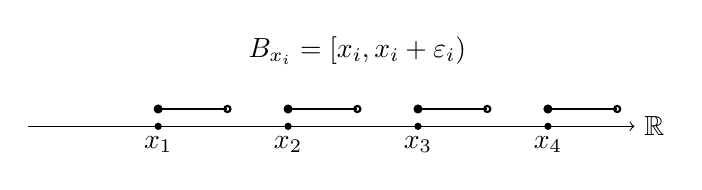
\begin{tikzpicture}[scale=1.1]
  % Eje real
  \draw[->] (-0.5,0) -- (6.5,0) node[right] {$\mathbb{R}$};

  % Puntos x1, x2, x3
  \foreach \x in {1,2.5,4,5.5}{
    \filldraw[black] (\x,0) circle (1pt);
  }
  \node[below] at (1,0) {$x_1$};
  \node[below] at (2.5,0) {$x_2$};
  \node[below] at (4,0) {$x_3$};
  \node[below] at (5.5,0) {$x_4$};

  % Intervalos semiabiertos [x, x+ε)
  \foreach \x in {1,2.5,4,5.5}{
    \draw[thick] (\x,0.2) -- (\x+0.8,0.2);
    \filldraw[black] (\x,0.2) circle (1.3pt);
    \draw[thick] (\x+0.8,0.2) circle (1pt);
  }

  % Etiqueta
  \node[above] at (3.3,0.6) {$B_{x_i} = [x_i, x_i+\varepsilon_i)$};
\end{tikzpicture}

\smallskip
\textit{Cada punto $x_i$ necesita su propio intervalo $[x_i, x_i+\varepsilon_i)$,
por lo que no puede haber una base numerable.}
\end{center}
\section*{$\mathbb{R}$ con la topología cofinita no es $1AN$}

Recordemos que en la topología cofinita de $\mathbb{R}$, los abiertos son:
\[
U \subseteq \mathbb{R} \quad \text{tales que} \quad \mathbb{R}\setminus U \text{ es finito.}
\]

\subsection*{Demostración (por reducción al absurdo)}

Supongamos que $\mathbb{R}$ con la topología cofinita satisface el primer axioma de numerabilidad (1AN).  
Entonces, para cada punto $x \in \mathbb{R}$, existe una base numerable de entornos $\{B_n(x)\}_{n\in\mathbb{N}}$.

\medskip
En particular, consideremos el punto $0$.  
Cada entorno básico de $0$ en la topología cofinita tiene la forma:
\[
B_n(0) = \mathbb{R} \setminus F_n,
\]
donde $F_n$ es un conjunto finito de puntos aislados.

\medskip
Queremos construir un entorno $B$ de $0$ que no contenga a ninguno de los $B_n(0)$.  
Para ello, basta con encontrar un punto que no pertenezca a ninguno de los conjuntos finitos $F_n$.

\[
F = \bigcup_{n\in\mathbb{N}} F_n
\]
es la unión numerable de conjuntos finitos, por tanto, $F$ es numerable.

\medskip
Como $\mathbb{R}$ no es numerable, existe un punto $x \in \mathbb{R} \setminus F$.  
Definimos el entorno:
\[
B = \mathbb{R} \setminus \{x\}.
\]
$B$ es abierto en la topología cofinita (su complemento $\{x\}$ es finito),  
pero no contiene ninguno de los $B_n(0)$, ya que ningún $B_n(0)$ elimina el punto $x$.

\medskip
Esto contradice la suposición de que $\{B_n(0)\}$ era una base de entornos en $0$.  
Por tanto, $\mathbb{R}$ con la topología cofinita \textbf{no cumple el primer axioma de numerabilidad}.

\[
\boxed{\mathbb{R}_{\text{cofinita}} \text{ no es } 1AN.}
\]
\section*{Un espacio es $T_1$ si y solo si los puntos son cerrados}

Sea $(X,\mathcal T)$ un espacio topológico.

\subsection*{($\Rightarrow$) Si $X$ es $T_1$, entonces $\{x\}$ es cerrado para todo $x\in X$}
Por $T_1$, para cada par $x\neq y$ existe un abierto $V_y$ tal que
\[
y\in V_y \quad\text{y}\quad x\notin V_y.
\]
Entonces
\[
X\setminus\{x\}=\bigcup_{y\in X\setminus\{x\}} V_y,
\]
es unión de abiertos, luego es abierto. Por tanto, su complementario $\{x\}$ es cerrado.

\subsection*{($\Leftarrow$) Si todo punto es cerrado, entonces $X$ es $T_1$}
Supongamos que cada $\{x\}$ es cerrado. Tomemos $x\neq y$.
Como $\{y\}$ es cerrado, $X\setminus\{y\}$ es abierto y contiene a $x$ pero no a $y$.
Simétricamente, $X\setminus\{x\}$ es abierto y contiene a $y$ pero no a $x$.
Esto verifica la condición $T_1$.
\section*{Densidad: $\overline{H}=X \iff H\cap A\neq\varnothing$ para todo abierto no vacío $A$}

Sea $(X,\mathcal T)$ un espacio topológico y $H\subseteq X$.

\subsection*{$(\Rightarrow)$ Si $\overline{H}=X$, entonces $H$ corta a todo abierto no vacío}
Supongamos, por absurdo, que existe un abierto no vacío $A\in\mathcal T$ tal que $H\cap A=\varnothing$.
Entonces $A\subseteq X\setminus H$, y como $A$ es abierto que no intersecta a $H$,
todo punto de $A$ tiene un entorno contenido en $X\setminus H$; por tanto
\[
A\subseteq X\setminus \overline{H},
\]
lo que contradice $\overline{H}=X$. Luego necesariamente $H\cap A\neq\varnothing$ para todo abierto no vacío $A$.

\subsection*{$(\Leftarrow)$ Si $H$ corta a todo abierto no vacío, entonces $\overline{H}=X$}
Supongamos, por absurdo, que existe $x\in X\setminus \overline{H}$.
Por definición de clausura, existe un abierto $U\in\mathcal T$ con
\[
x\in U \quad\text{y}\quad U\cap H=\varnothing.
\]
Pero $U$ es un abierto no vacío que no corta a $H$, contradicción con la hipótesis.
Luego no hay tal $x$ y, por tanto, $\overline{H}=X$.
\section*{Complemento de un conjunto no denso en ninguna parte es denso}

Sea $(X,\mathcal T)$ un espacio topológico y $A\subseteq X$.
Recordamos que $A$ es \emph{no denso en ninguna parte} si
\[
\operatorname{int}\big(\overline{A}\big)=\varnothing.
\]
El conjunto es solo frontera.
\subsection*{Teorema}
Si $A$ es no denso en ninguna parte, entonces $X\setminus A$ es denso en $X$.

\subsection*{Demostración}
Primero probamos que $X\setminus\overline{A}$ es abierto y denso.
Es evidente que $X\setminus\overline{A}$ es abierto. Para ver que es denso,
tomemos un abierto no vacío $U\subseteq X$. Si ocurriera
$U\cap (X\setminus\overline{A})=\varnothing$, entonces $U\subseteq \overline{A}$,
lo cual implicaría $U\subseteq \operatorname{int}(\overline{A})$, contradiciendo
$\operatorname{int}(\overline{A})=\varnothing$. Por tanto,
todo abierto $U$ corta a $X\setminus\overline{A}$ y éste es denso.

Como $X\setminus A \supseteq X\setminus\overline{A}$, se tiene
\[
\overline{\,X\setminus A\,}\ \supseteq\ \overline{\,X\setminus\overline{A}\,}\ =\ X,
\]
luego $X\setminus A$ es denso.

\end{document}